\documentclass[../notes.tex]{subfiles}

\pagestyle{main}
\renewcommand{\chaptermark}[1]{\markboth{\chaptername\ \thechapter\ (#1)}{}}
\setcounter{chapter}{2}

\begin{document}




\chapter{Cyclic Intermediates}
\section{Problems 1, 2, 3, 4, 5, and 6}
\begin{itemize}
    \item \marginnote{9/13:}We begin with Problem 3.
    \begin{figure}[h!]
        \centering
        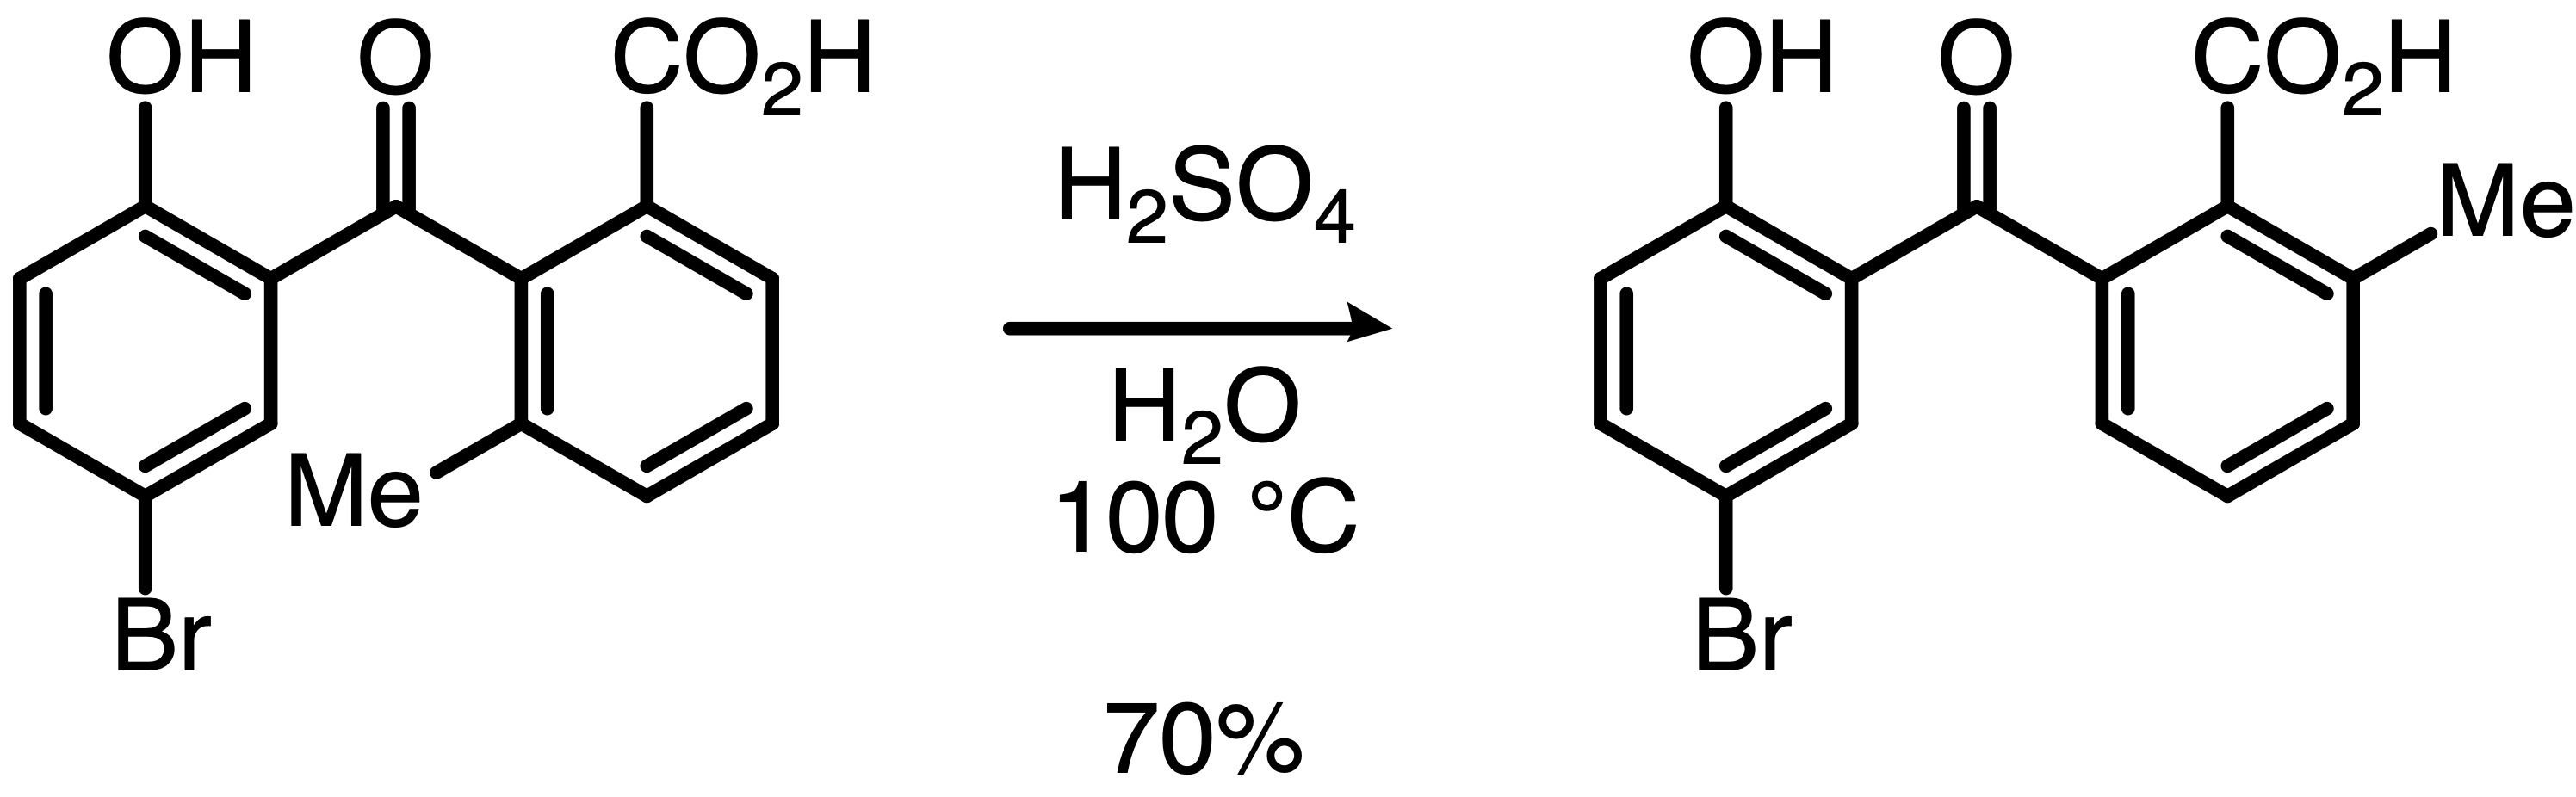
\includegraphics[width=0.45\linewidth]{MPSet3Q3.png}
        \caption{Movassaghi PSet 3, Q3.}
        \label{fig:MPSet3Q3}
    \end{figure}
    \item Fairly acidic conditions; fairly high temperature. So fairly forcing.
    \item First step could be electrophilic aromatic substitution. In Friedel-Crafts, the $\pi$-system acts as a nucleophile.
    \item We go through a spiro-fused bicycle juncture. Without the methyl group, it'd be fully symmetric.
    \item You can't acylate an aromatic system with a carboxylic acid.
    \item To get to an acylium ion in the starting material, protonate at the less favored position of the carboxylic acid \ce{OH}. This will happen at 1 in a billion molecules, and that's what the forcing conditions get us. Then water leaves.
    \item Ask myself: What sites could you protonate, and where would this get us?
    \begin{itemize}
        \item Reversible protonation of the carbonyl does nothing, so move on.
        \item Few reagents implies an intramolecular reaction.
        \item In an intramolecular reaction, think about which atoms could go where without something breaking off fully.
    \end{itemize}
    \item The \ce{OH} of the phenol could hydrogen-bond to the carbonyl and planarize the system.
    \item Dearomatizing the ring is uphill. The bonds will be fairly labile. This first step could well go backwards! The point is that pretty much every step here is reversible. But why do we get dominant formation of the product?
    \begin{itemize}
        \item The left molecule (with two ortho substituents) has rotation about the right phenyl-carbonyl bond. With the prodcut substituents, the molecule can be planar and we get additional stabilization via full conjugation.
    \end{itemize}
    \item In Friedel-Crafts chemistry, phenols are ortho- and para-directing, so remember that our phenol can have some nucleophilicity.
    \item Altogether, the full solution to PSet 3, Q3 is on the next page.
    \begin{figure}[h!]
        \centering
        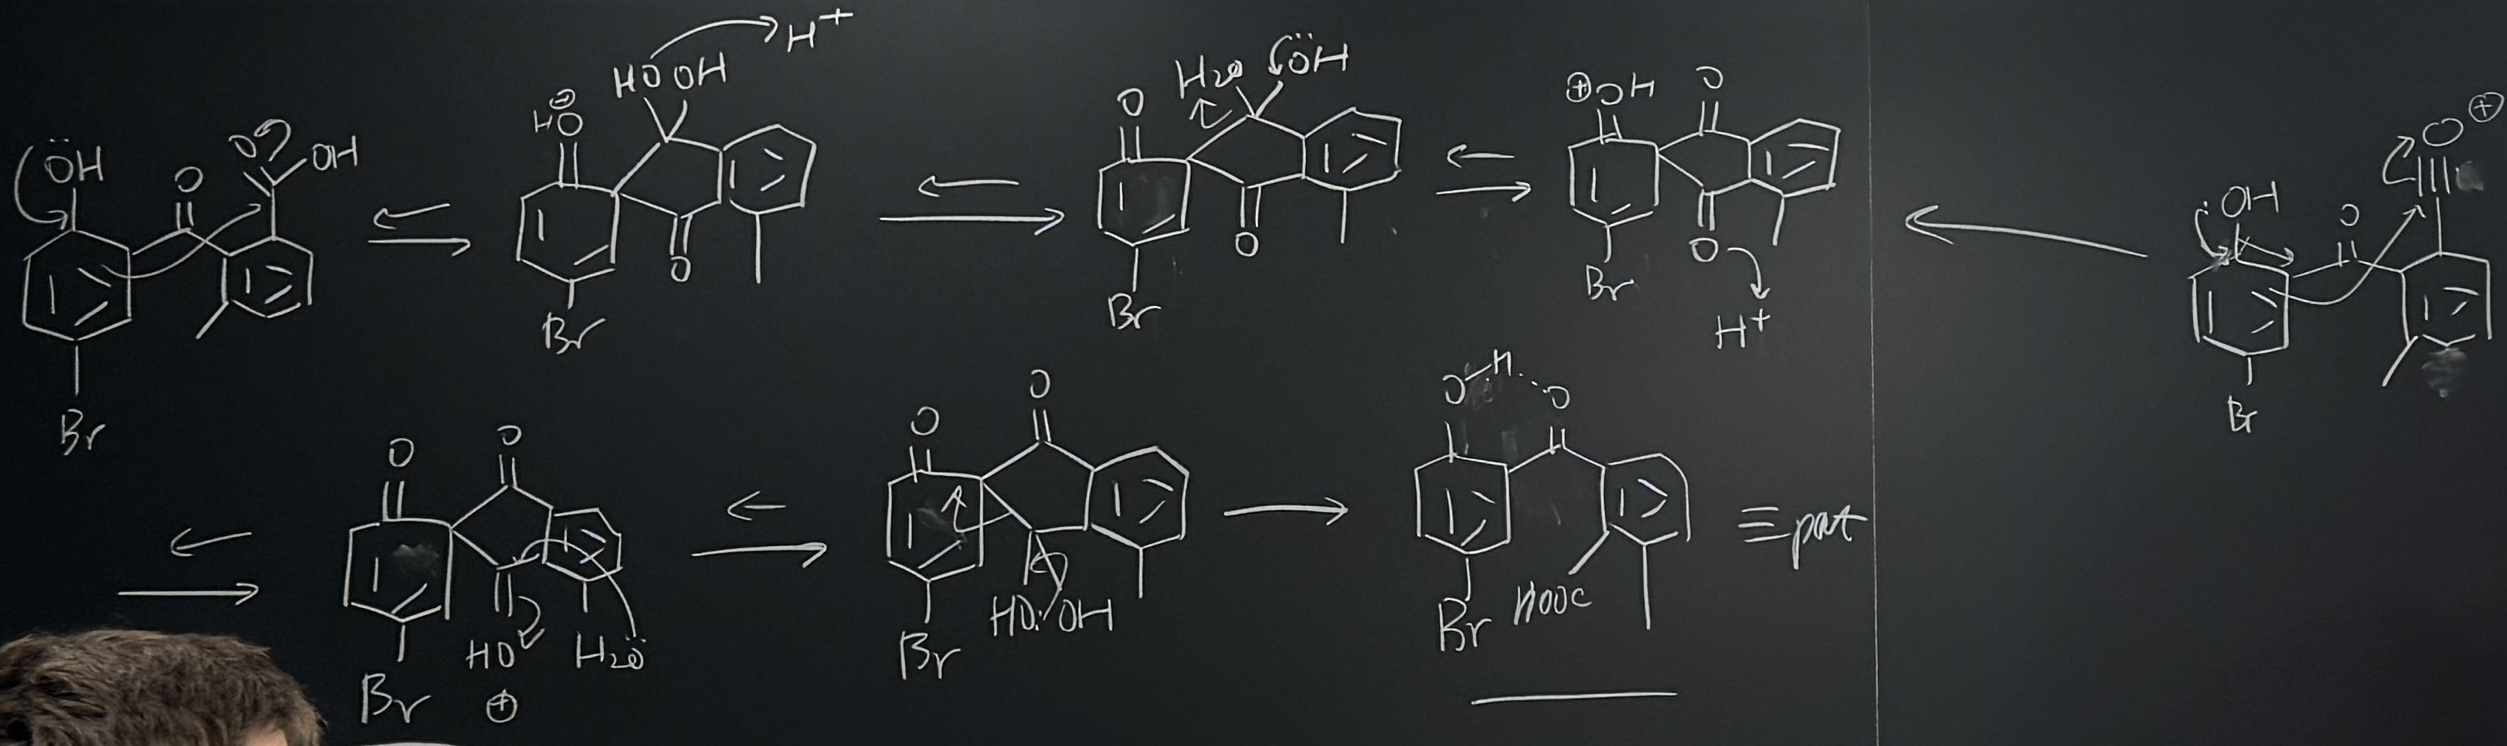
\includegraphics[width=0.8\linewidth]{MPSet3Q3S.JPG}
        \caption{Movassaghi PSet 3, Q3 solution.}
        \label{fig:MPSet3Q3S}
    \end{figure}
    \pagebreak
    \item We now begin discussing Problem 1.
    \begin{figure}[h!]
        \centering
        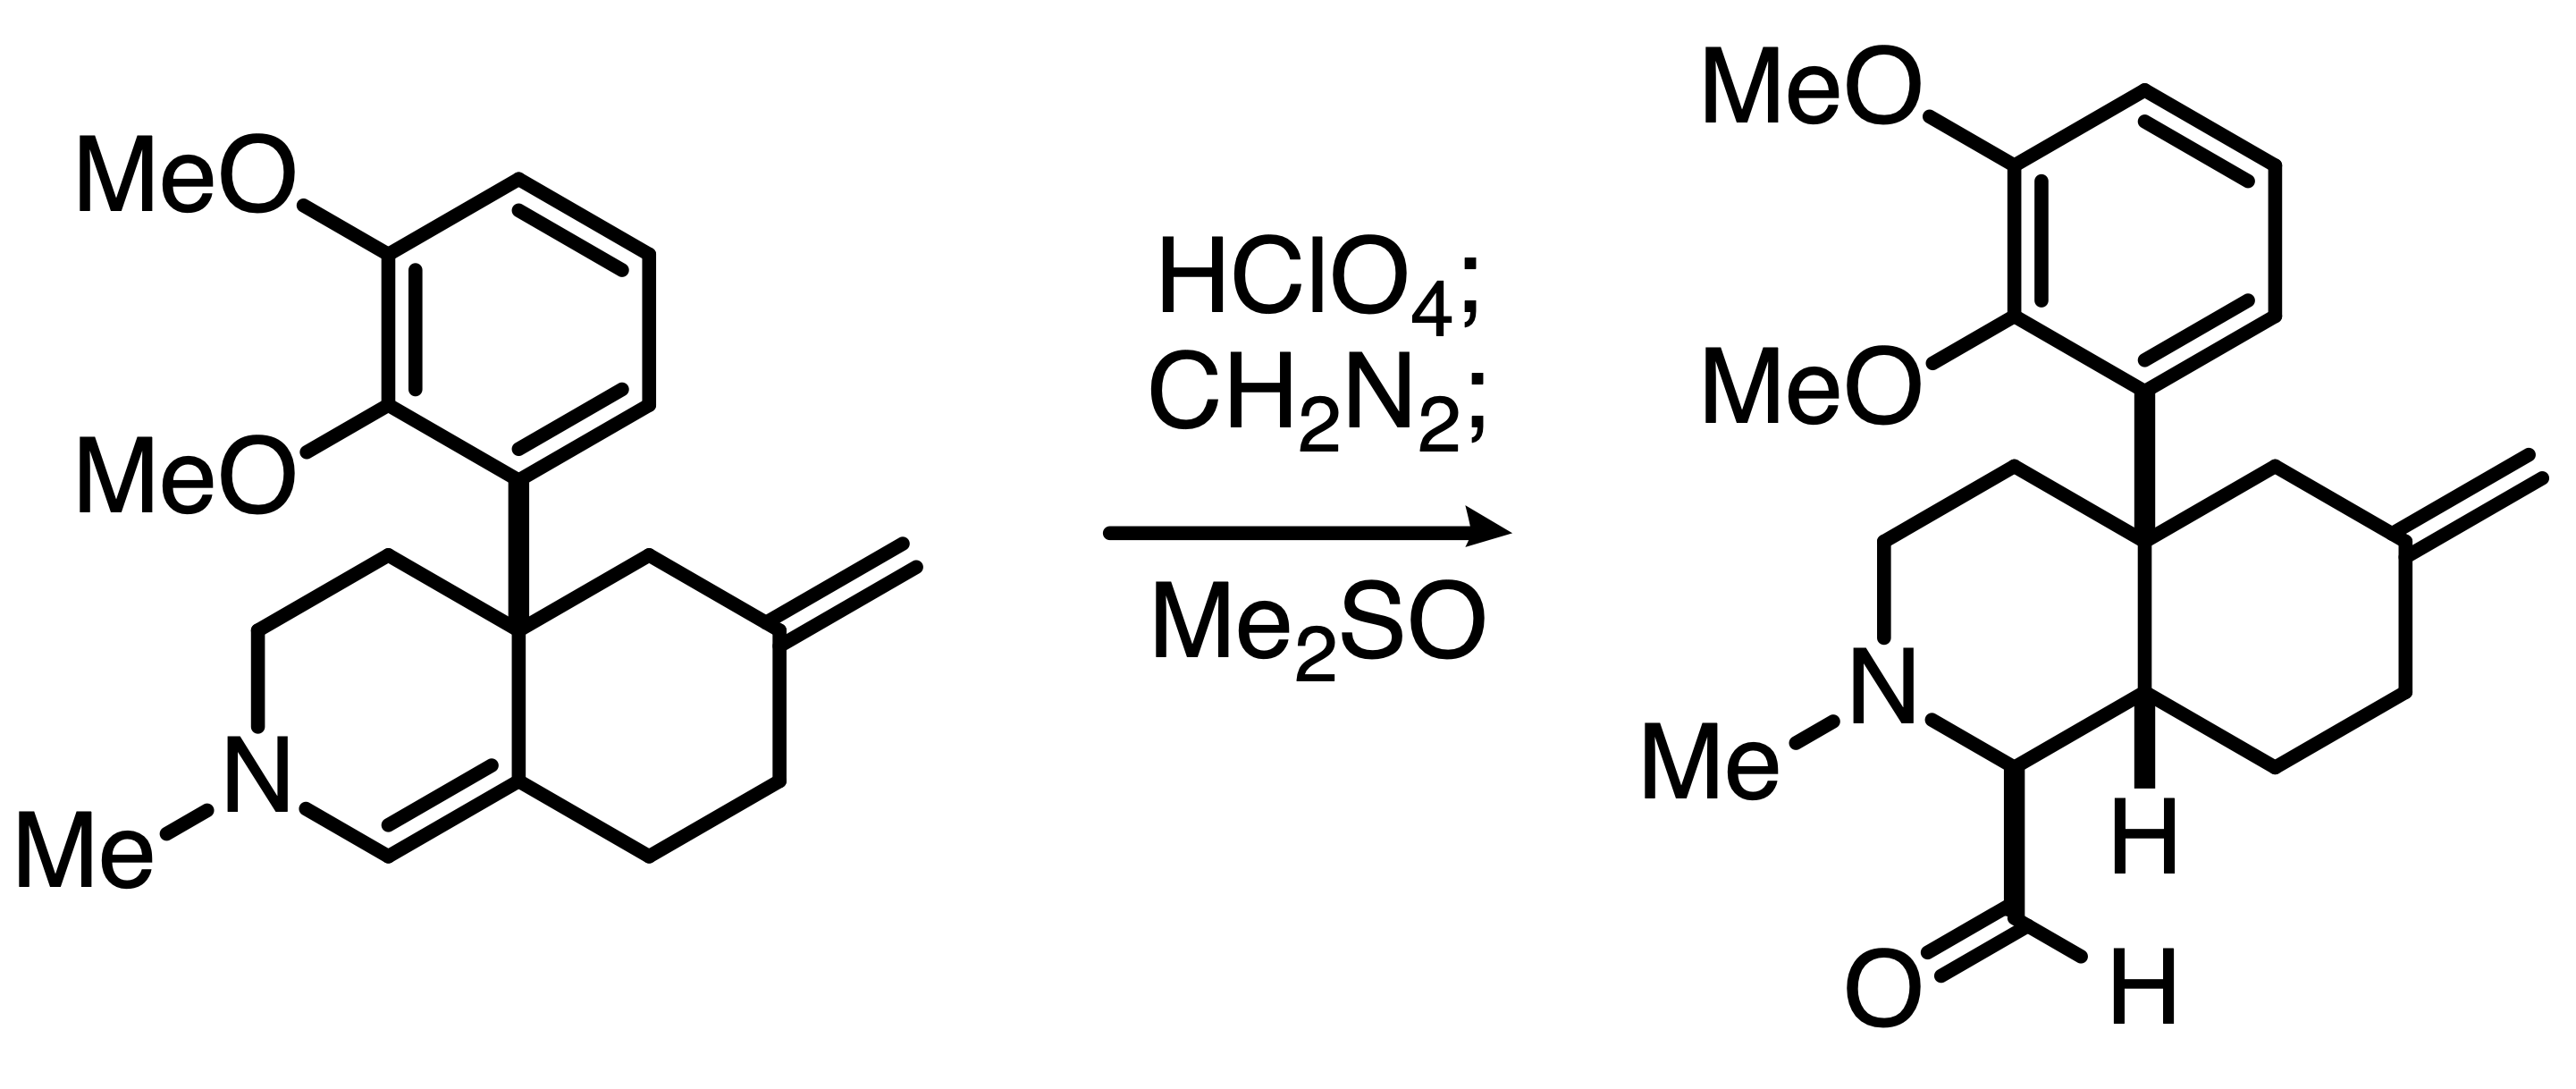
\includegraphics[width=0.4\linewidth]{MPSet3Q1.png}
        \caption{Movassaghi PSet 3, Q1.}
        \label{fig:MPSet3Q1}
    \end{figure}
    \item Perchloric acid is a very strong acid with a weak, nonnucleophilic counterion. Thus, protonation is correct.
    \item However, what protonating the enamine might not be favorable.
    \begin{itemize}
        \item The enamine is more nucleophilic than the enol because the nitrogen can stabilize positive charge better than the oxygen.
        \item Lone pair donation to the enamine will override any alkene selectivity.
        \item This is why we protonate the tertiary position.
    \end{itemize}
    \item Then the nucleophilic diazomethane attacks the iminium.
    \item Losing dinitrogen provides the energy you need to form a three membered aziridinium.
    \item Aziridine $\to$ aziridinium intermediate.
    \begin{itemize}
        \item Thus, nucleophilic addition and rupture of one of the bonds could relieve ring strain.
    \end{itemize}
    \item The DMSO oxygen attacks the less sterically hindered position.
    \item Positively charged sulfur has perchlorate as a counteranion.
    \item We don't need oxalyl chloride because we already have the key intermediate.
    \item Swern: The triethylamine actually deprotonates at the methyne; then the carbanion diprotonates at the ipso carbon.
    \begin{itemize}
        \item Retro $[3+2]$ dipolar cycloaddition.
        \item Involvement of ylides??
    \end{itemize}
    \item The methylamine in the structure can act as internal base; we could also have another molecule come by to do the deprotonation.
    \item Protonating the bicycle will lead to either a \emph{cis}-decalin derivative or a \emph{trans}-decalin derivative.
    \begin{itemize}
        \item The \emph{cis}-decalin has the aryl group being equatorial, which is energetically favorable.
        \item The aryl is not 1,3-interacting with the bottom ring because the double bond is bending the 3-hydrogen away.
        \item The approach coming from the top of diazomethane is much more favorable, because it's less hindered by the inside/underside of the \emph{cis}-decalin.
    \end{itemize}
    \item We should consider the stereochemistry at each step, because it impacts what chemical options are available at each step.
    \item Altogether, the full solution to PSet 3, Q1 is on the next page.
    \begin{figure}[H]
        \centering
        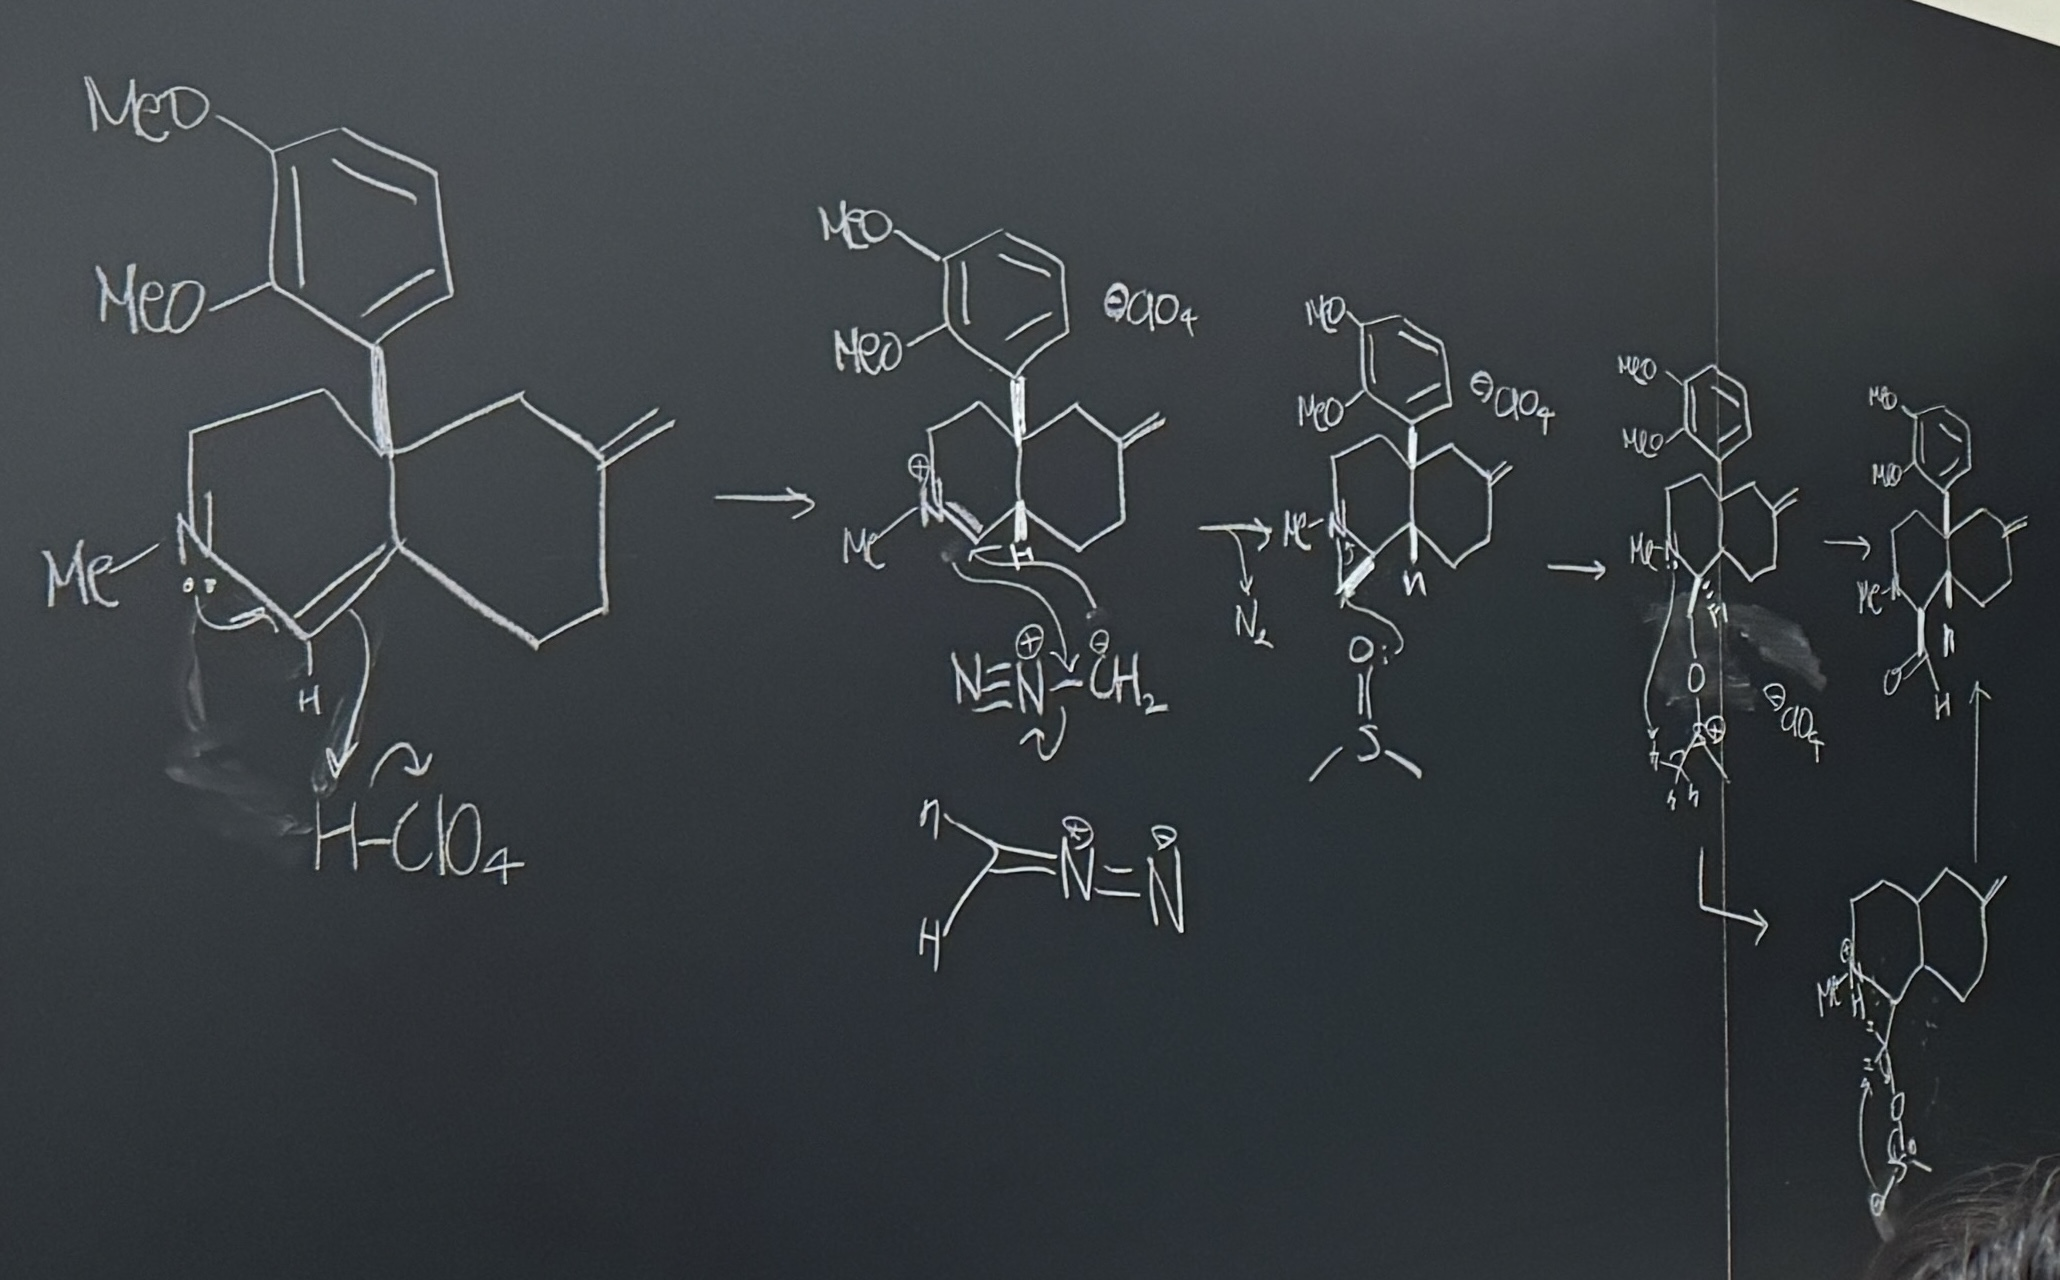
\includegraphics[width=0.8\linewidth]{MPSet3Q1S.JPG}
        \caption{Movassaghi PSet 3, Q1 solution.}
        \label{fig:MPSet3Q1S}
    \end{figure}
    \pagebreak
    \item We now begin discussing Problem 4.
    \begin{figure}[h!]
        \centering
        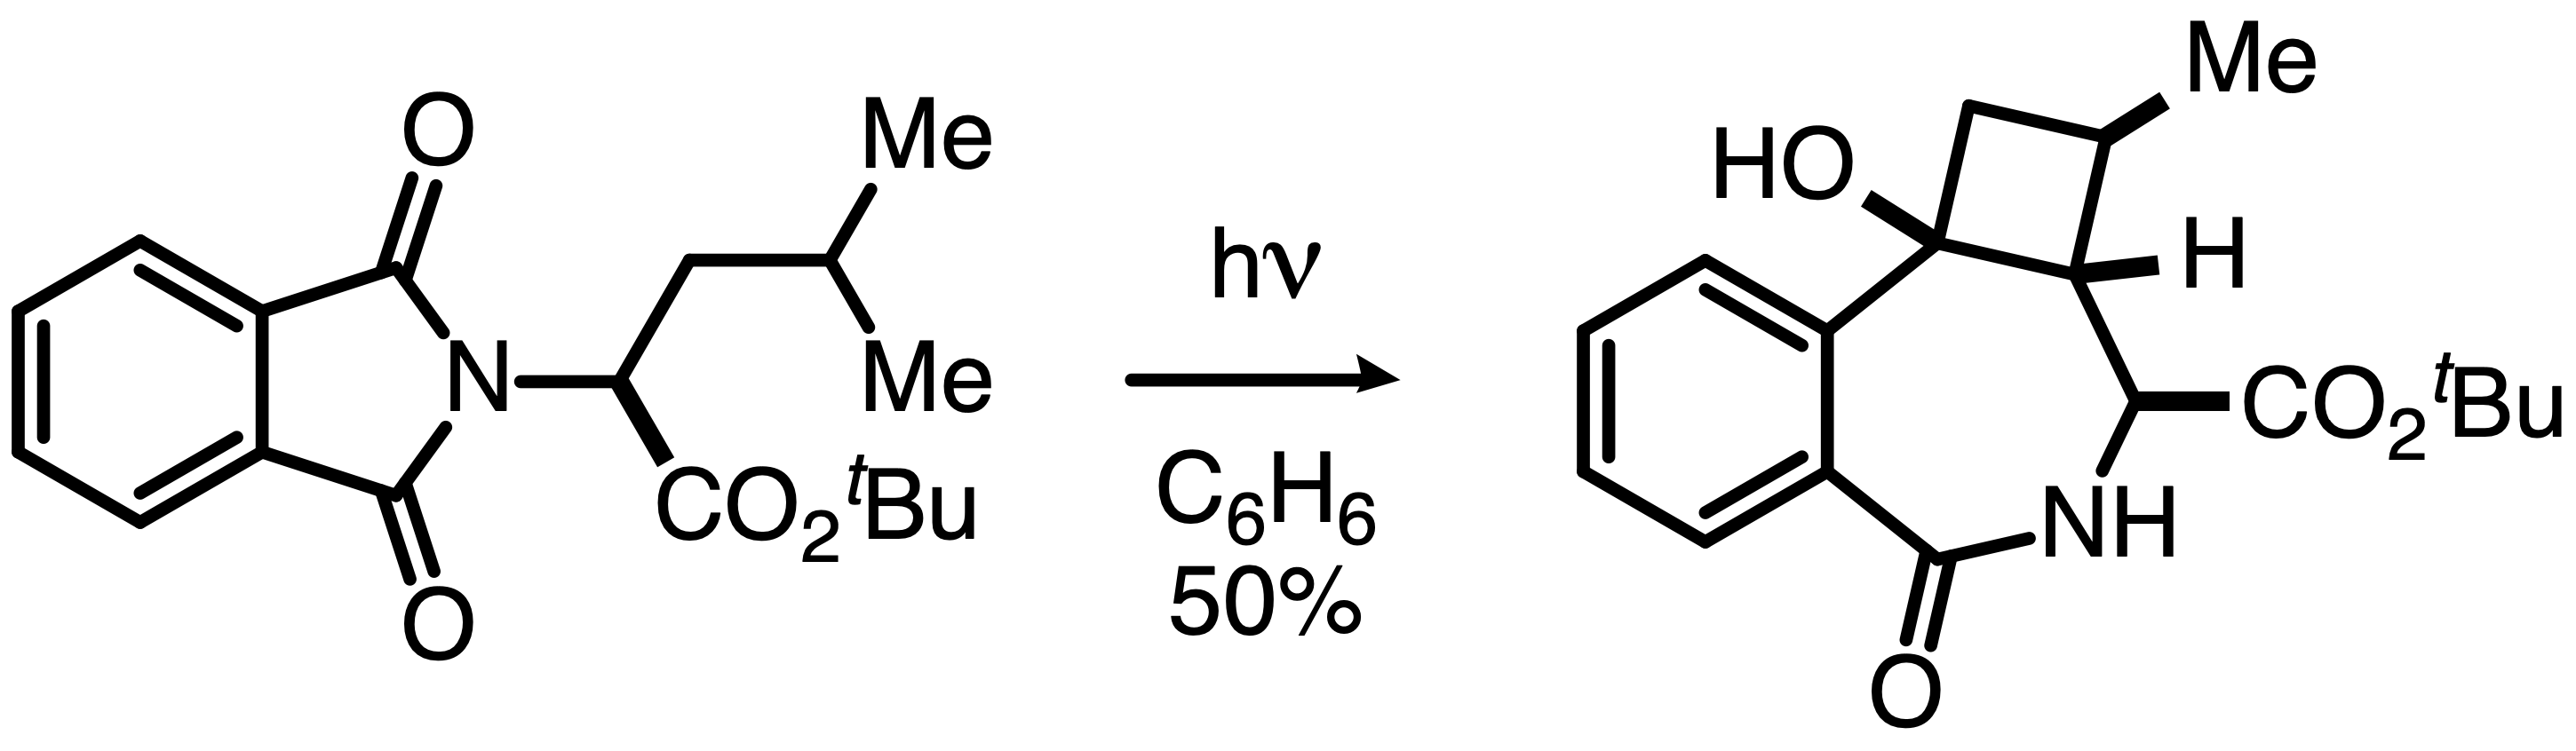
\includegraphics[width=0.45\linewidth]{MPSet3Q4.png}
        \caption{Movassaghi PSet 3, Q4.}
        \label{fig:MPSet3Q4}
    \end{figure}
    \item Photoexcitation makes the carbonyl into a diradical. Then we have 1,5-H atom abstraction (which is optimal, as we've discussed previously).
    \begin{itemize}
        \item We will photoexcite either of the two carbonyls in the phthalimide.
        \item It's easier to photoexcite conjugated systems because we've got a larger box (particle in a box QM analogy). Larger boxes have lower excitation energy. \emph{check the math!!}
        \item Once you photoexcite the carbonyl, you'll go back, do $\alpha$-cleavage to form an acyl radical, or do 1,5-H atom abstraction.
        \item David: Where is the intersystem crossing?
        \begin{itemize}
            \item Singlets or triplets can form a bond; the aromatic system will help enable the ISC exchange.
        \end{itemize}
    \end{itemize}
    \item Two carbon radicals quickly form a 4-membered ring, driven by killing radicals and forming a \ce{C-C} $\sigma$-bond.
    \begin{itemize}
        \item The 4-membered ring is an azocyclobutane.
    \end{itemize}
    \item Then we get another 1,5-H atom abstraction, and another ring-closing reaction.
    \item Altogether, the full solution to PSet 3, Q4 is on the next page.
    \begin{figure}[H]
        \centering
        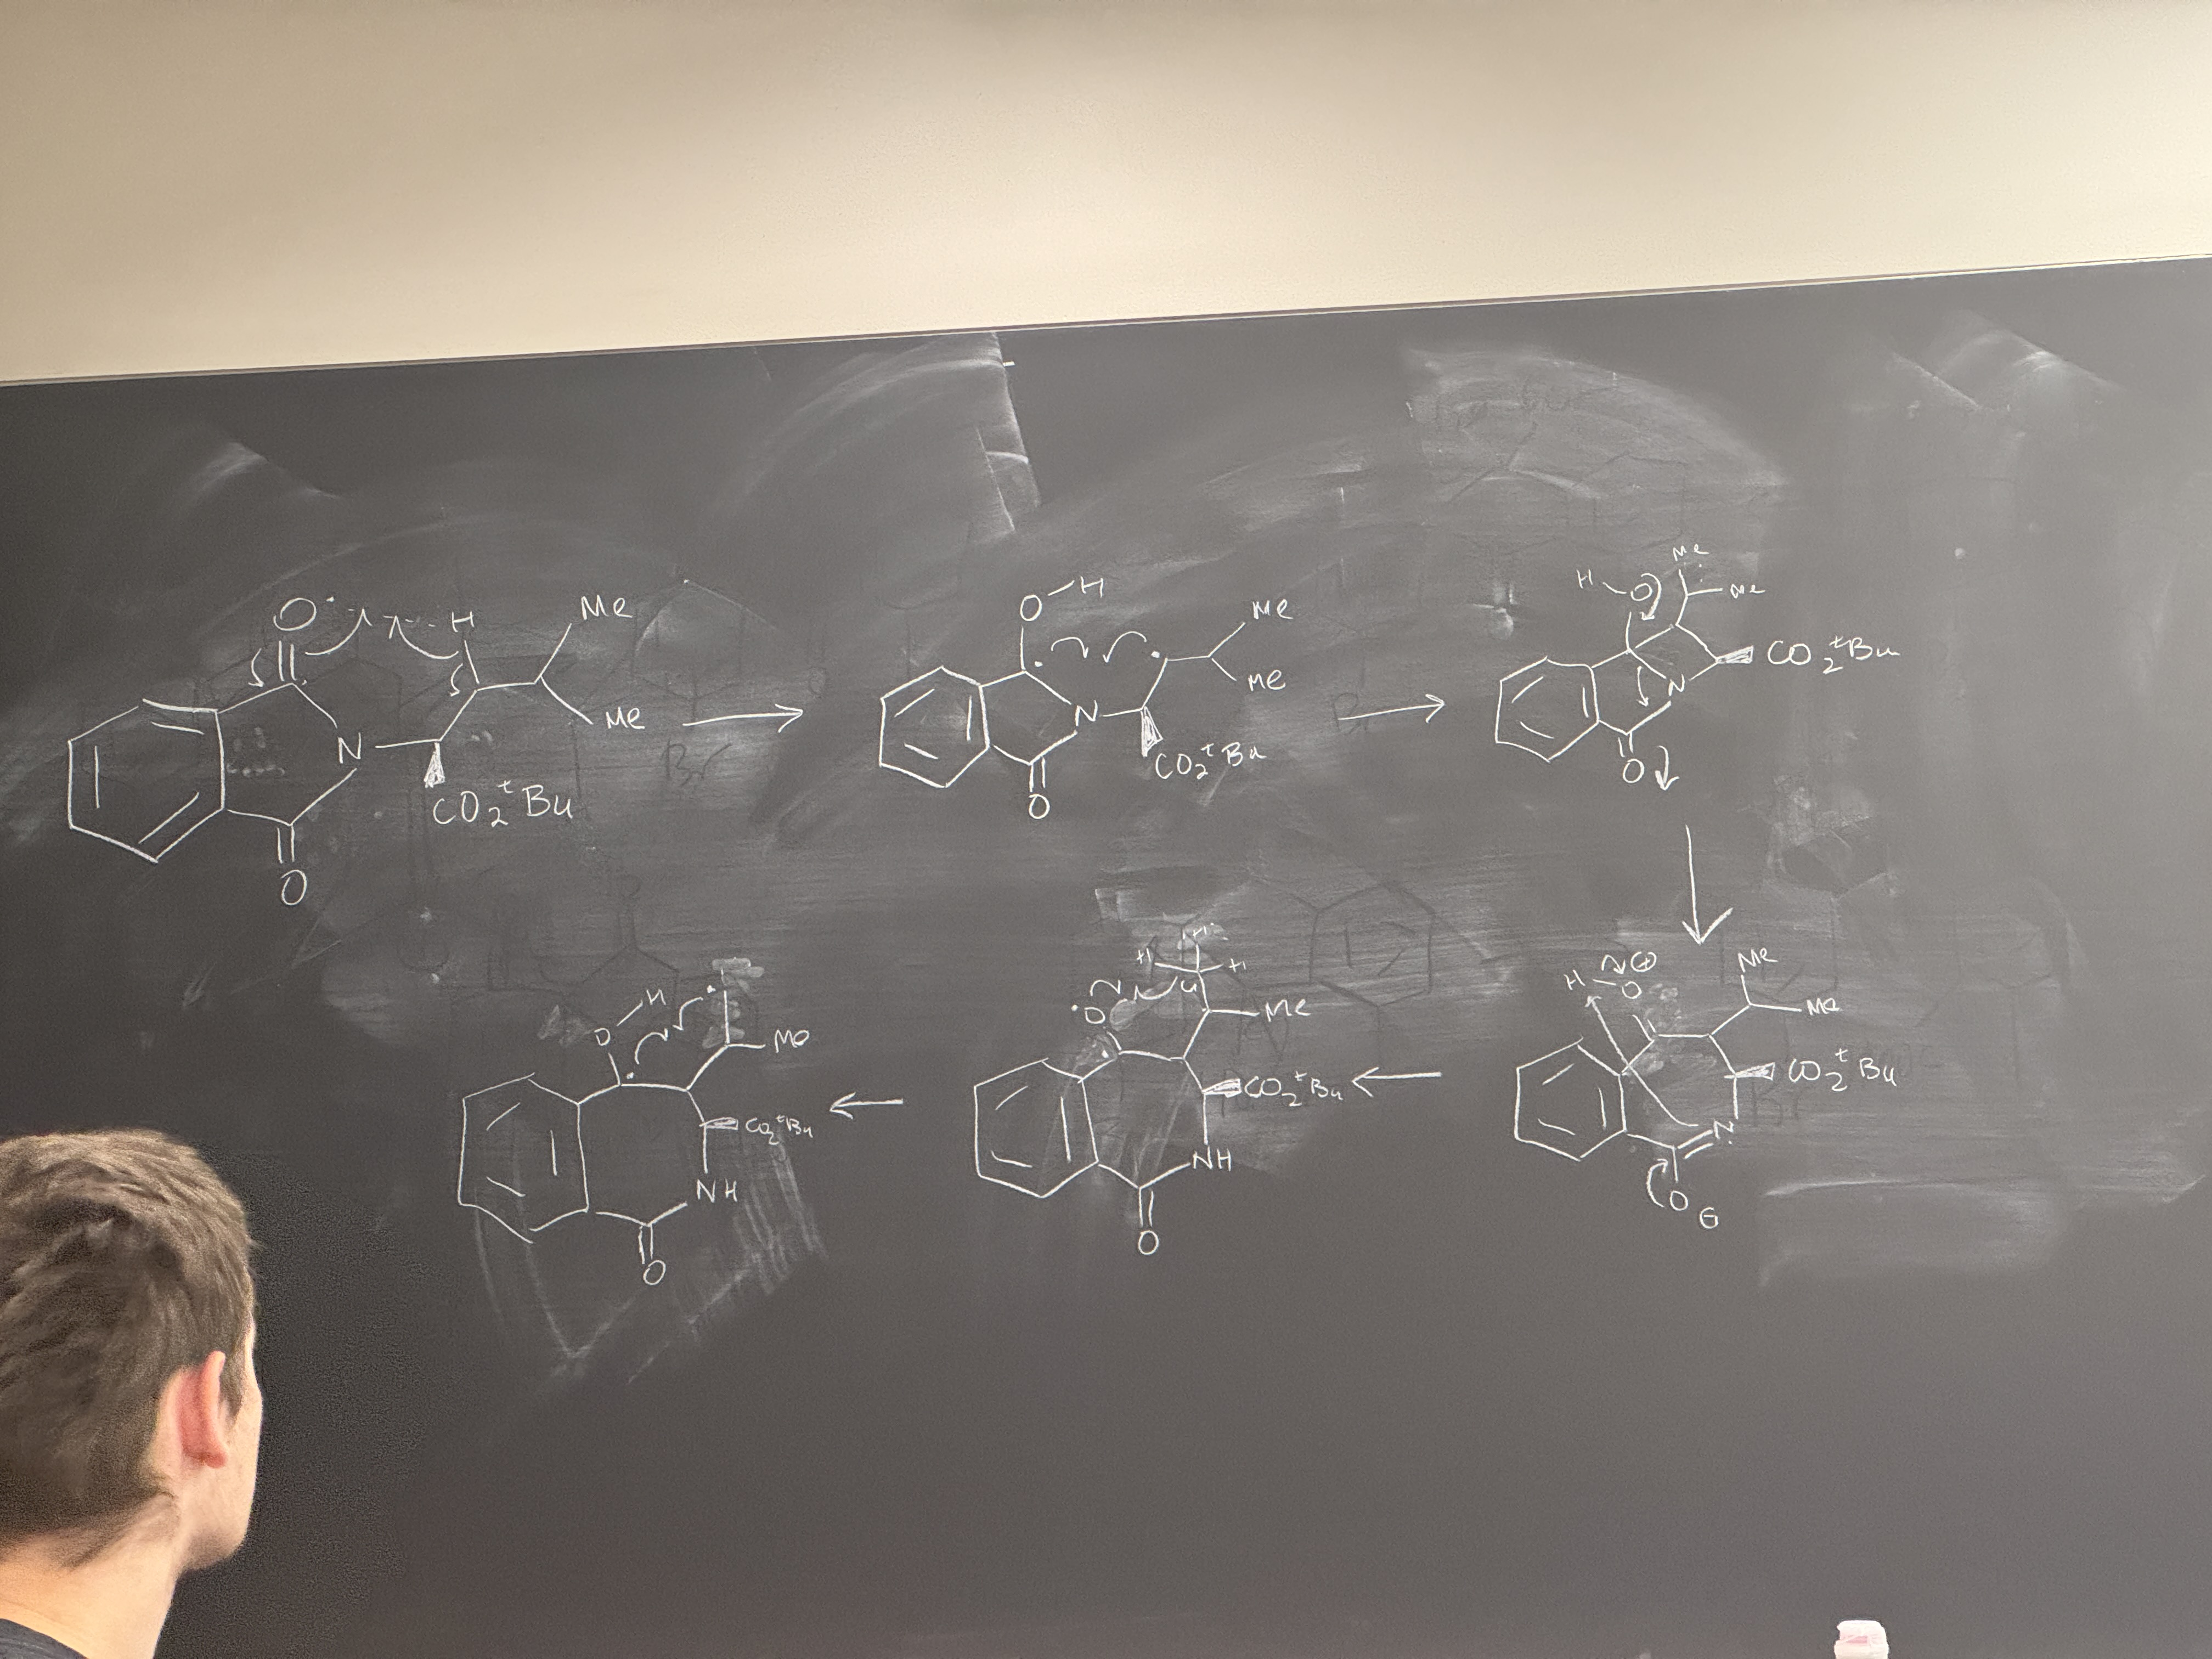
\includegraphics[width=0.8\linewidth]{MPSet3Q4S.JPG}
        \caption{Movassaghi PSet 3, Q4 solution.}
        \label{fig:MPSet3Q4S}
    \end{figure}
    \pagebreak
    \item We now begin discussing Problem 2.
    \begin{figure}[h!]
        \centering
        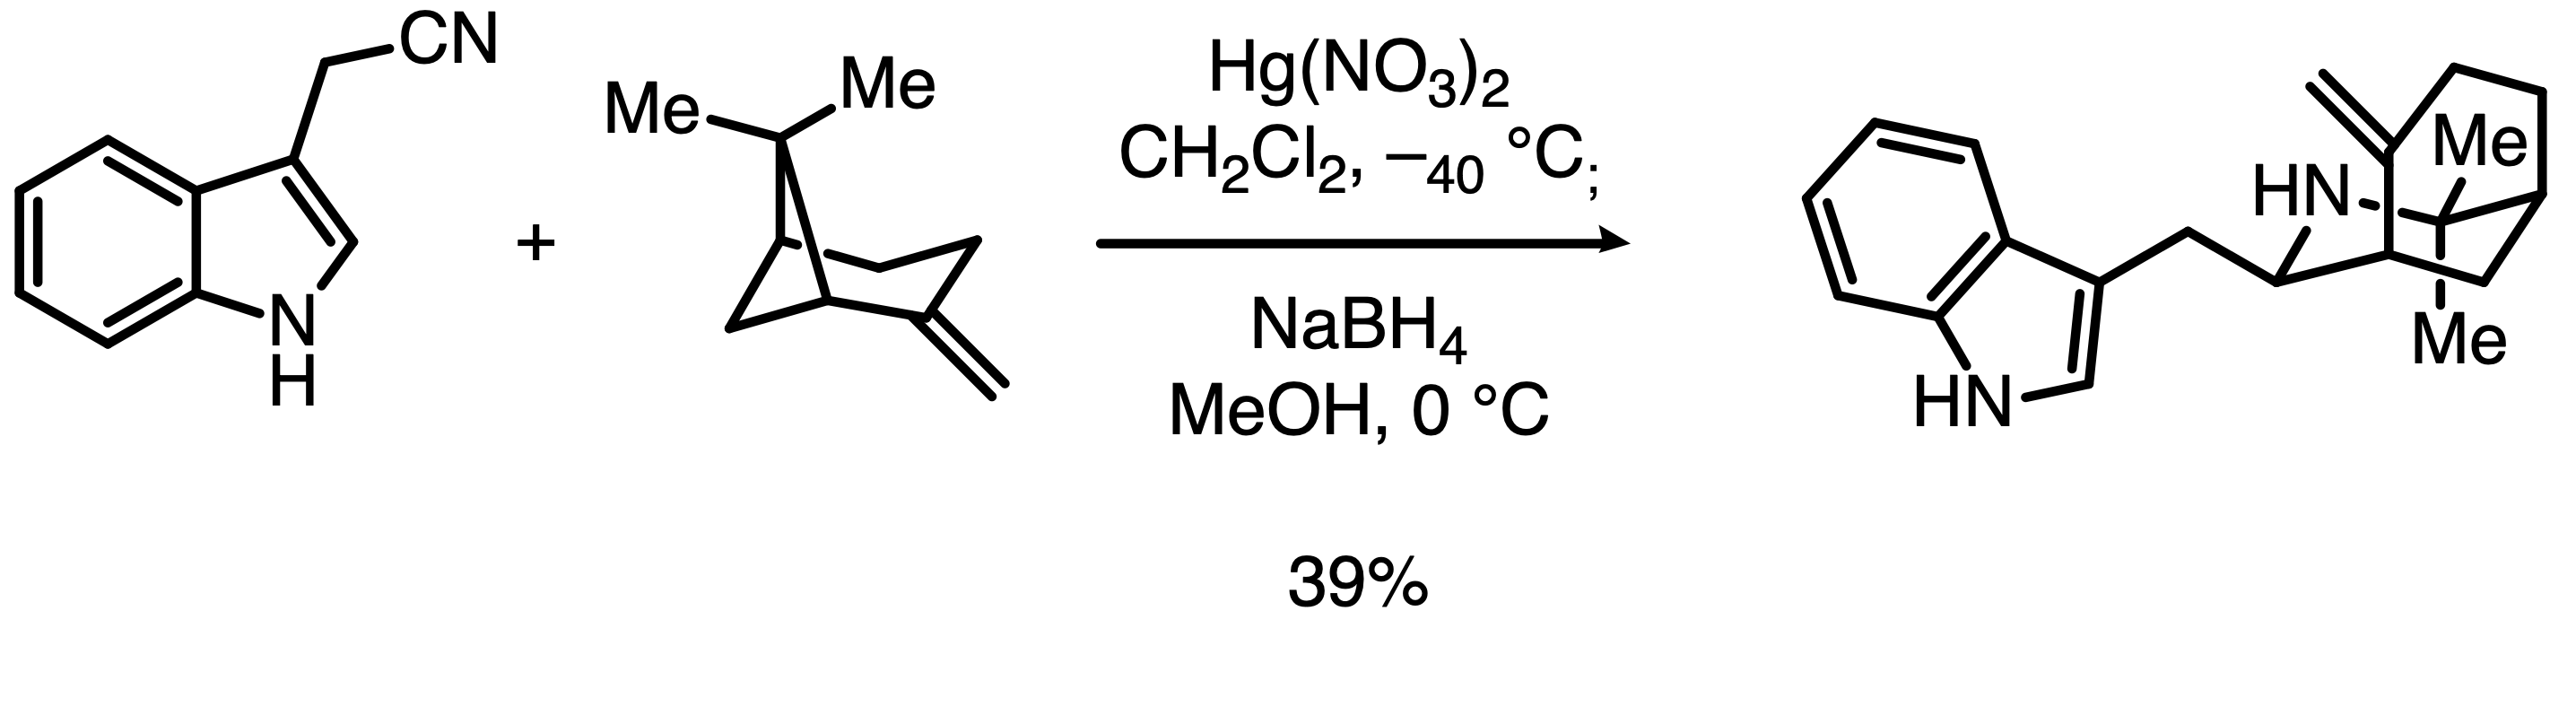
\includegraphics[width=0.6\linewidth]{MPSet3Q2.png}
        \caption{Movassaghi PSet 3, Q2.}
        \label{fig:MPSet3Q2}
    \end{figure}
    \item Look at quaternary carbons as places that a \ce{C-C} $\sigma$-bond could leave behind a carbocation.
    \item We form the mercurinium ion.
    \begin{itemize}
        \item The tertiary carbocation is less stable than the mercurinium ion.
        \item Focus on what's reversible.
        \item Releasing ring strain drives the formation of the tertiary carbocation.
        \item We need an antiperiplanar orientation between the \ce{C-C} bond that's breaking and the \ce{C-Hg} bond that's breaking.
        \item If mercury attacked from the top: (1) that's less likely due to steric bulk at the top of the molecule, and it would just have to reverse because no antiperiplanar orientation for the shift.
    \end{itemize}
    \item Nitrilium ion has $\pKa=-10$.
    \item An analysis of pyrrole.
    \begin{itemize}
        \item Protonating it: Positive charge is on 1, 2, or 3 atoms.
        \item The most nucleophilic position is the $\alpha$-carbon.
    \end{itemize}
    \item Indole is just a variant of pyrrole. Indoles are very nucleophilic at the $\beta$-position.
    \item Thus, the indole nitrile is not the most nucleophilic species, but it is the most kinetically accessible.
    \item Indolyl group wants to be equatorial.
    \item Better to just kick out the mercury than use its lone pair.
    \begin{itemize}
        \item Look up oxymercuration mechanism!!
    \end{itemize}
    \item This reaction is a report of Clayton-Hithcock, even though it has mechanistic similarities to the Ritter reaction.
    \item Altogether, the full solution to PSet 3, Q2 is on the next page.
    \begin{figure}[H]
        \centering
        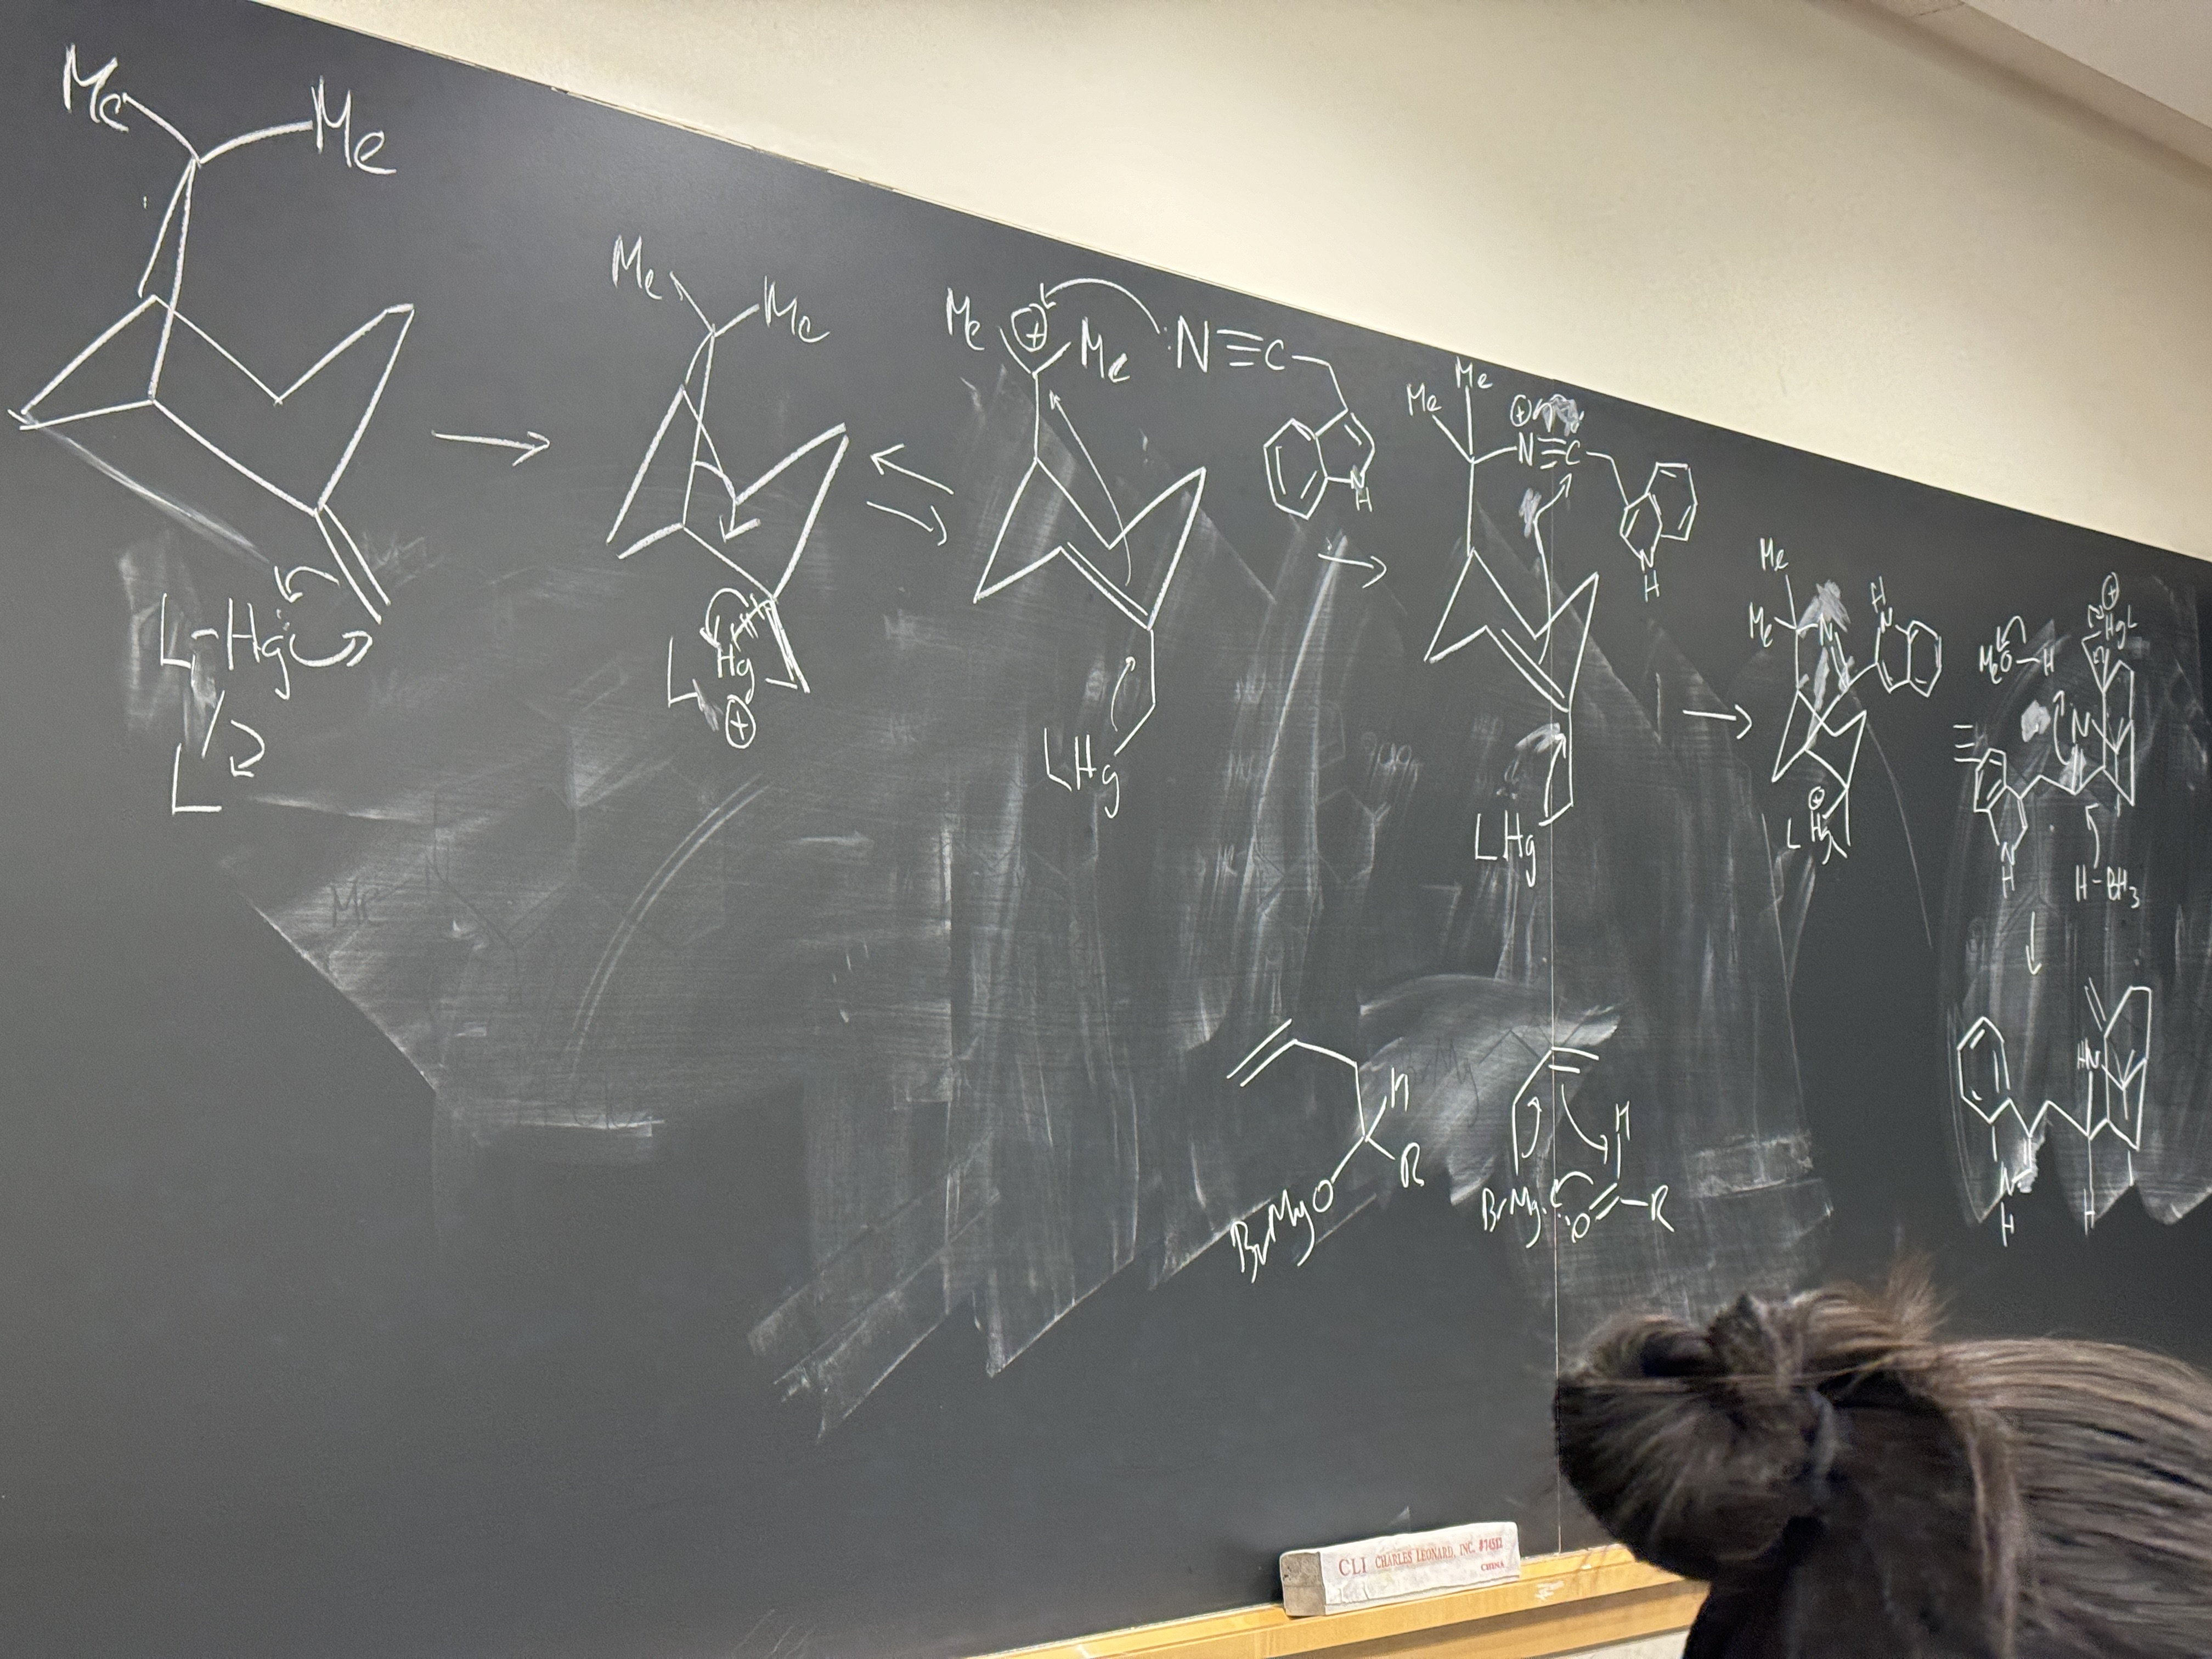
\includegraphics[width=0.8\linewidth]{MPSet3Q2S.JPG}
        \caption{Movassaghi PSet 3, Q2 solution.}
        \label{fig:MPSet3Q2S}
    \end{figure}
    \pagebreak
    \item We now begin discussing Problem 5.
    \begin{figure}[h!]
        \centering
        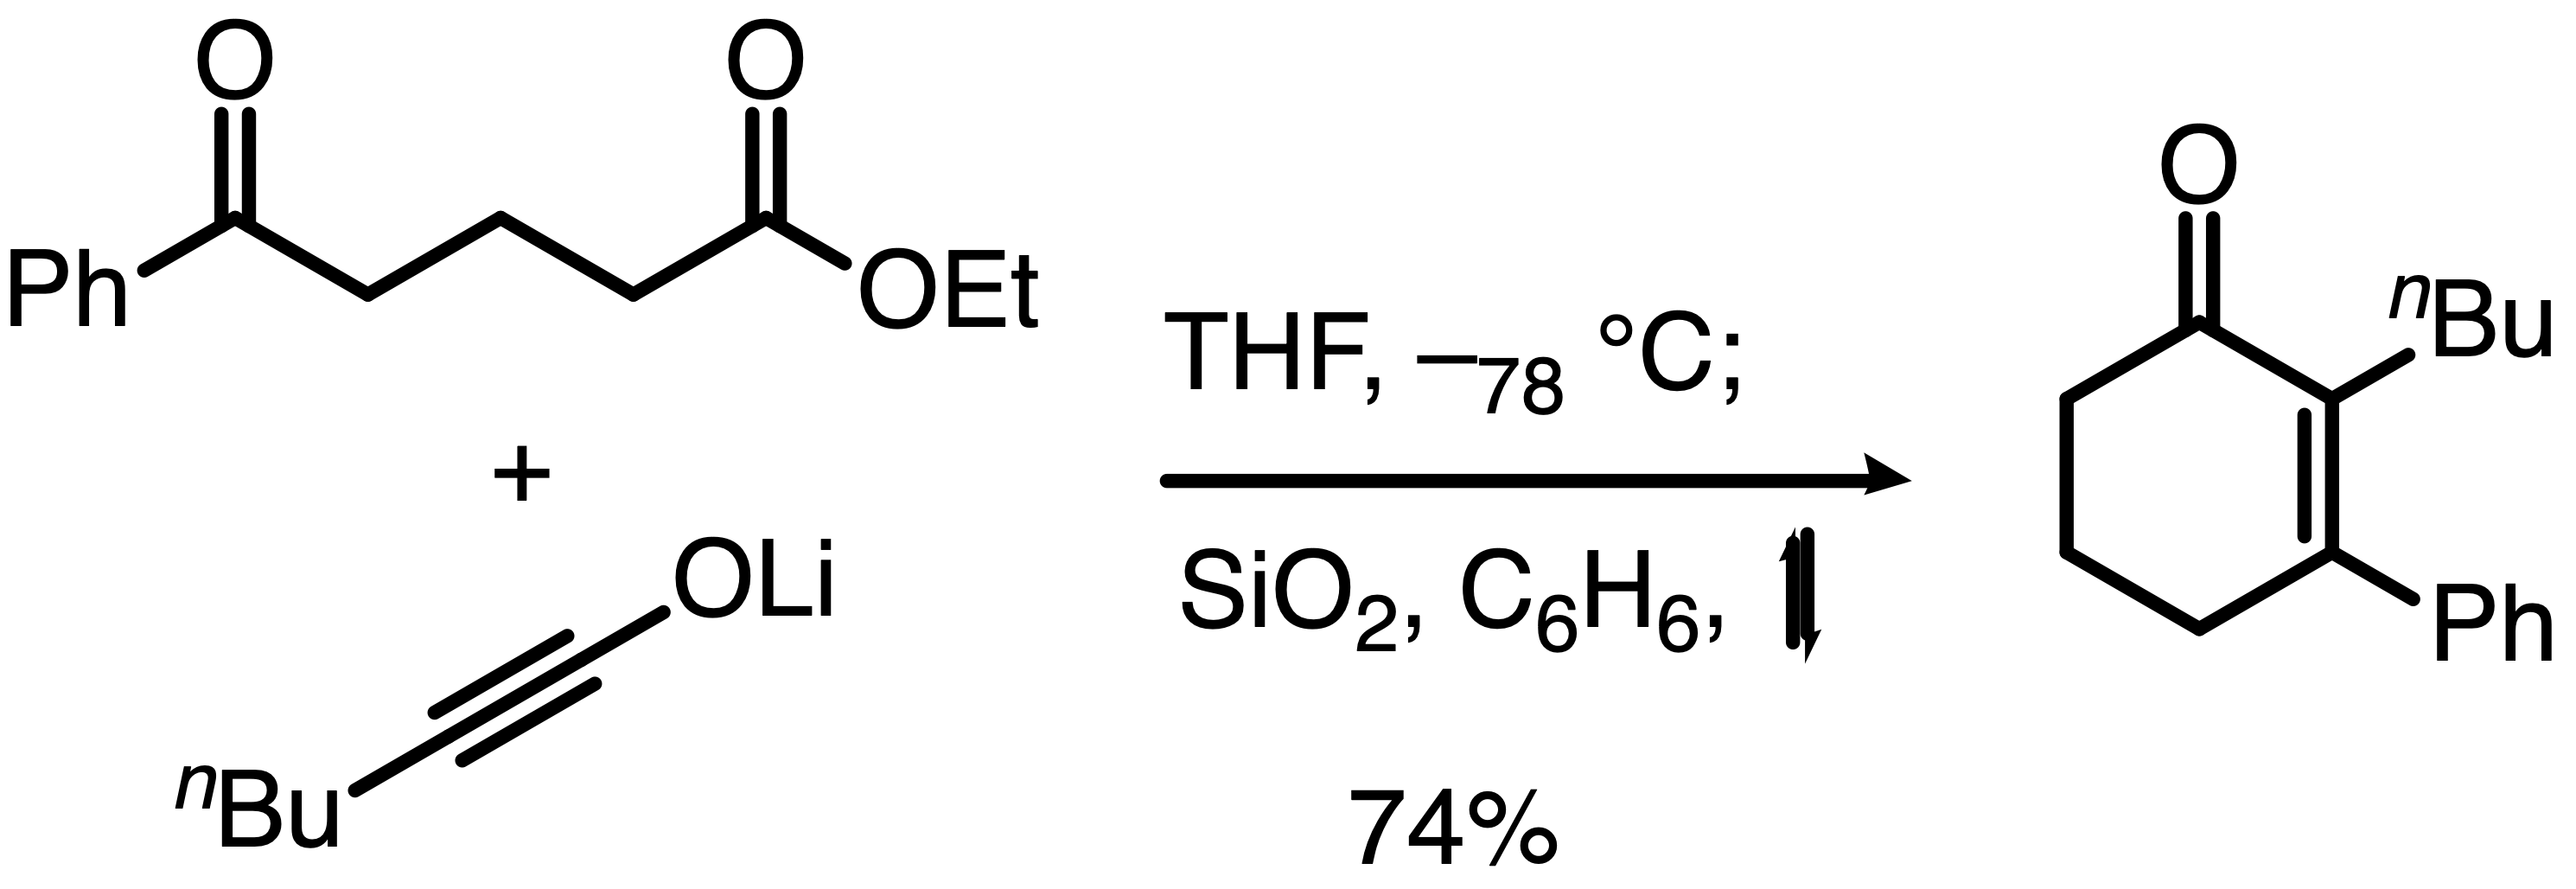
\includegraphics[width=0.4\linewidth]{MPSet3Q5.png}
        \caption{Movassaghi PSet 3, Q5.}
        \label{fig:MPSet3Q5}
    \end{figure}
    \item The ynolate could react like an enolate, but more likely it will be a concerted $[2+2]$ cycloaddition. Good to keep the counteranion on the oxygen to assist in the cycloassition.
    \item The reaction stops at the lactone in the first step. Then the addition of the acid, benzene, and heat weakens bonds and drives off \ce{CO2}.
    \item Altogether, the full solution to PSet 3, Q5 is on the next page.
    \begin{figure}[h!]
        \centering
        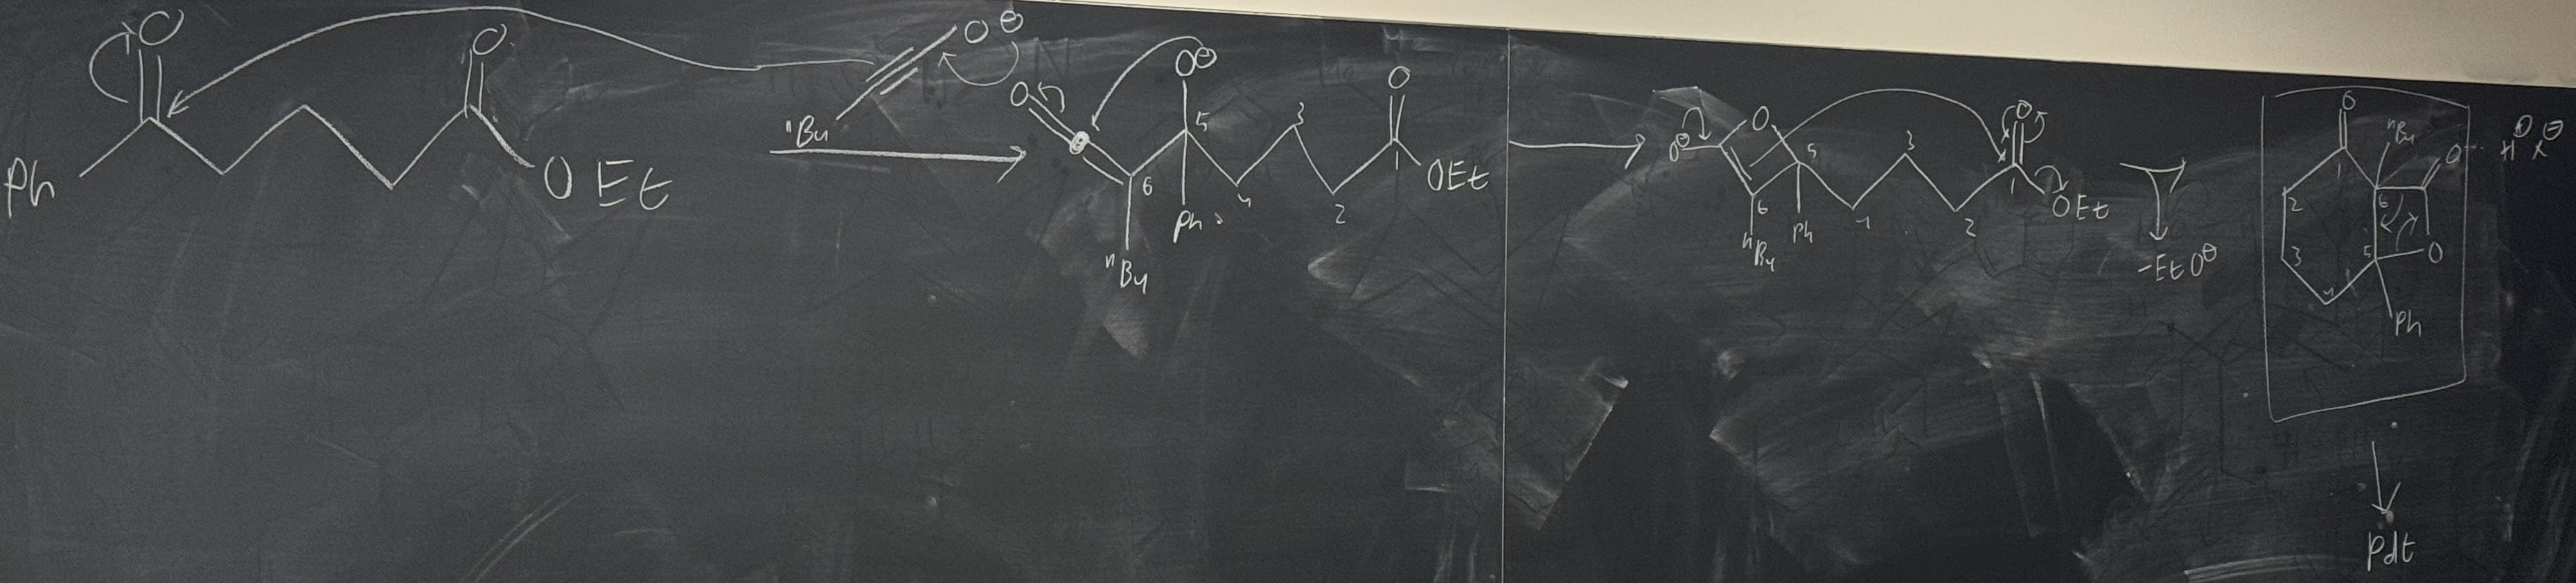
\includegraphics[width=0.8\linewidth]{MPSet3Q5S.JPG}
        \caption{Movassaghi PSet 3, Q5 solution.}
        \label{fig:MPSet3Q5S}
    \end{figure}
    \pagebreak
    \item We now begin discussing Problem 6.
    \begin{figure}[h!]
        \centering
        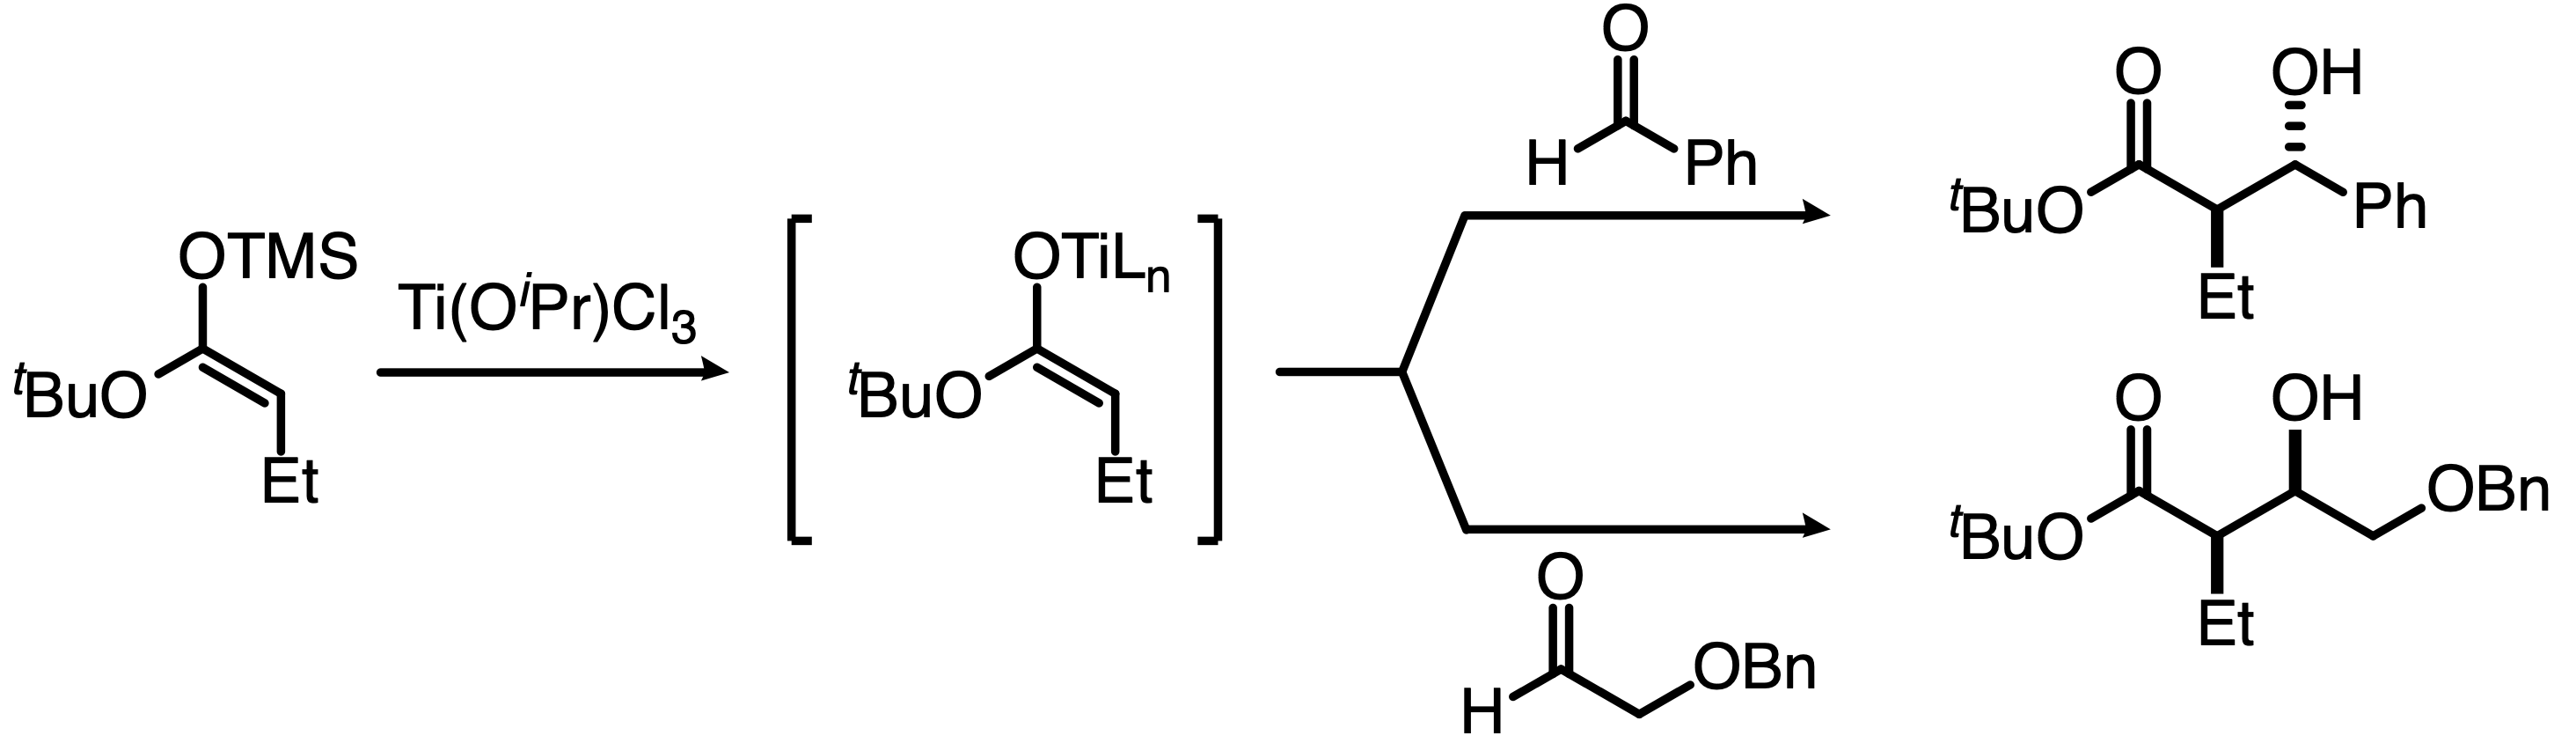
\includegraphics[width=0.7\linewidth]{MPSet3Q6.png}
        \caption{Movassaghi PSet 3, Q6.}
        \label{fig:MPSet3Q6}
    \end{figure}
    \item First step is just a deprotection.
    \item Then the transition state is a six-membered ring.
    \begin{itemize}
        \item Closed transition states: \textbf{Zimmerman-Traxler transition states}. Dave Evans helped a lot with understanding this reactivity!
    \end{itemize}
    \item What does the Lewis acid do?
    \begin{itemize}
        \item The aldehyde becomes more electrophilic if we put a Lewis acid on the oxygen. When they coordinate to titanium, they become more electrophilic.
        \item If something coordinates to the titanium, this also reactivates the enolate!
        \item This is \textbf{dual activation}, leading to maximum rate enhancement. This is a very important concept in boron chemistry: We'll come back to it in 5.511
    \end{itemize}
    \item Altogether, the full solution to PSet 3, Q6 is on the next page.
    \begin{figure}[h!]
        \centering
        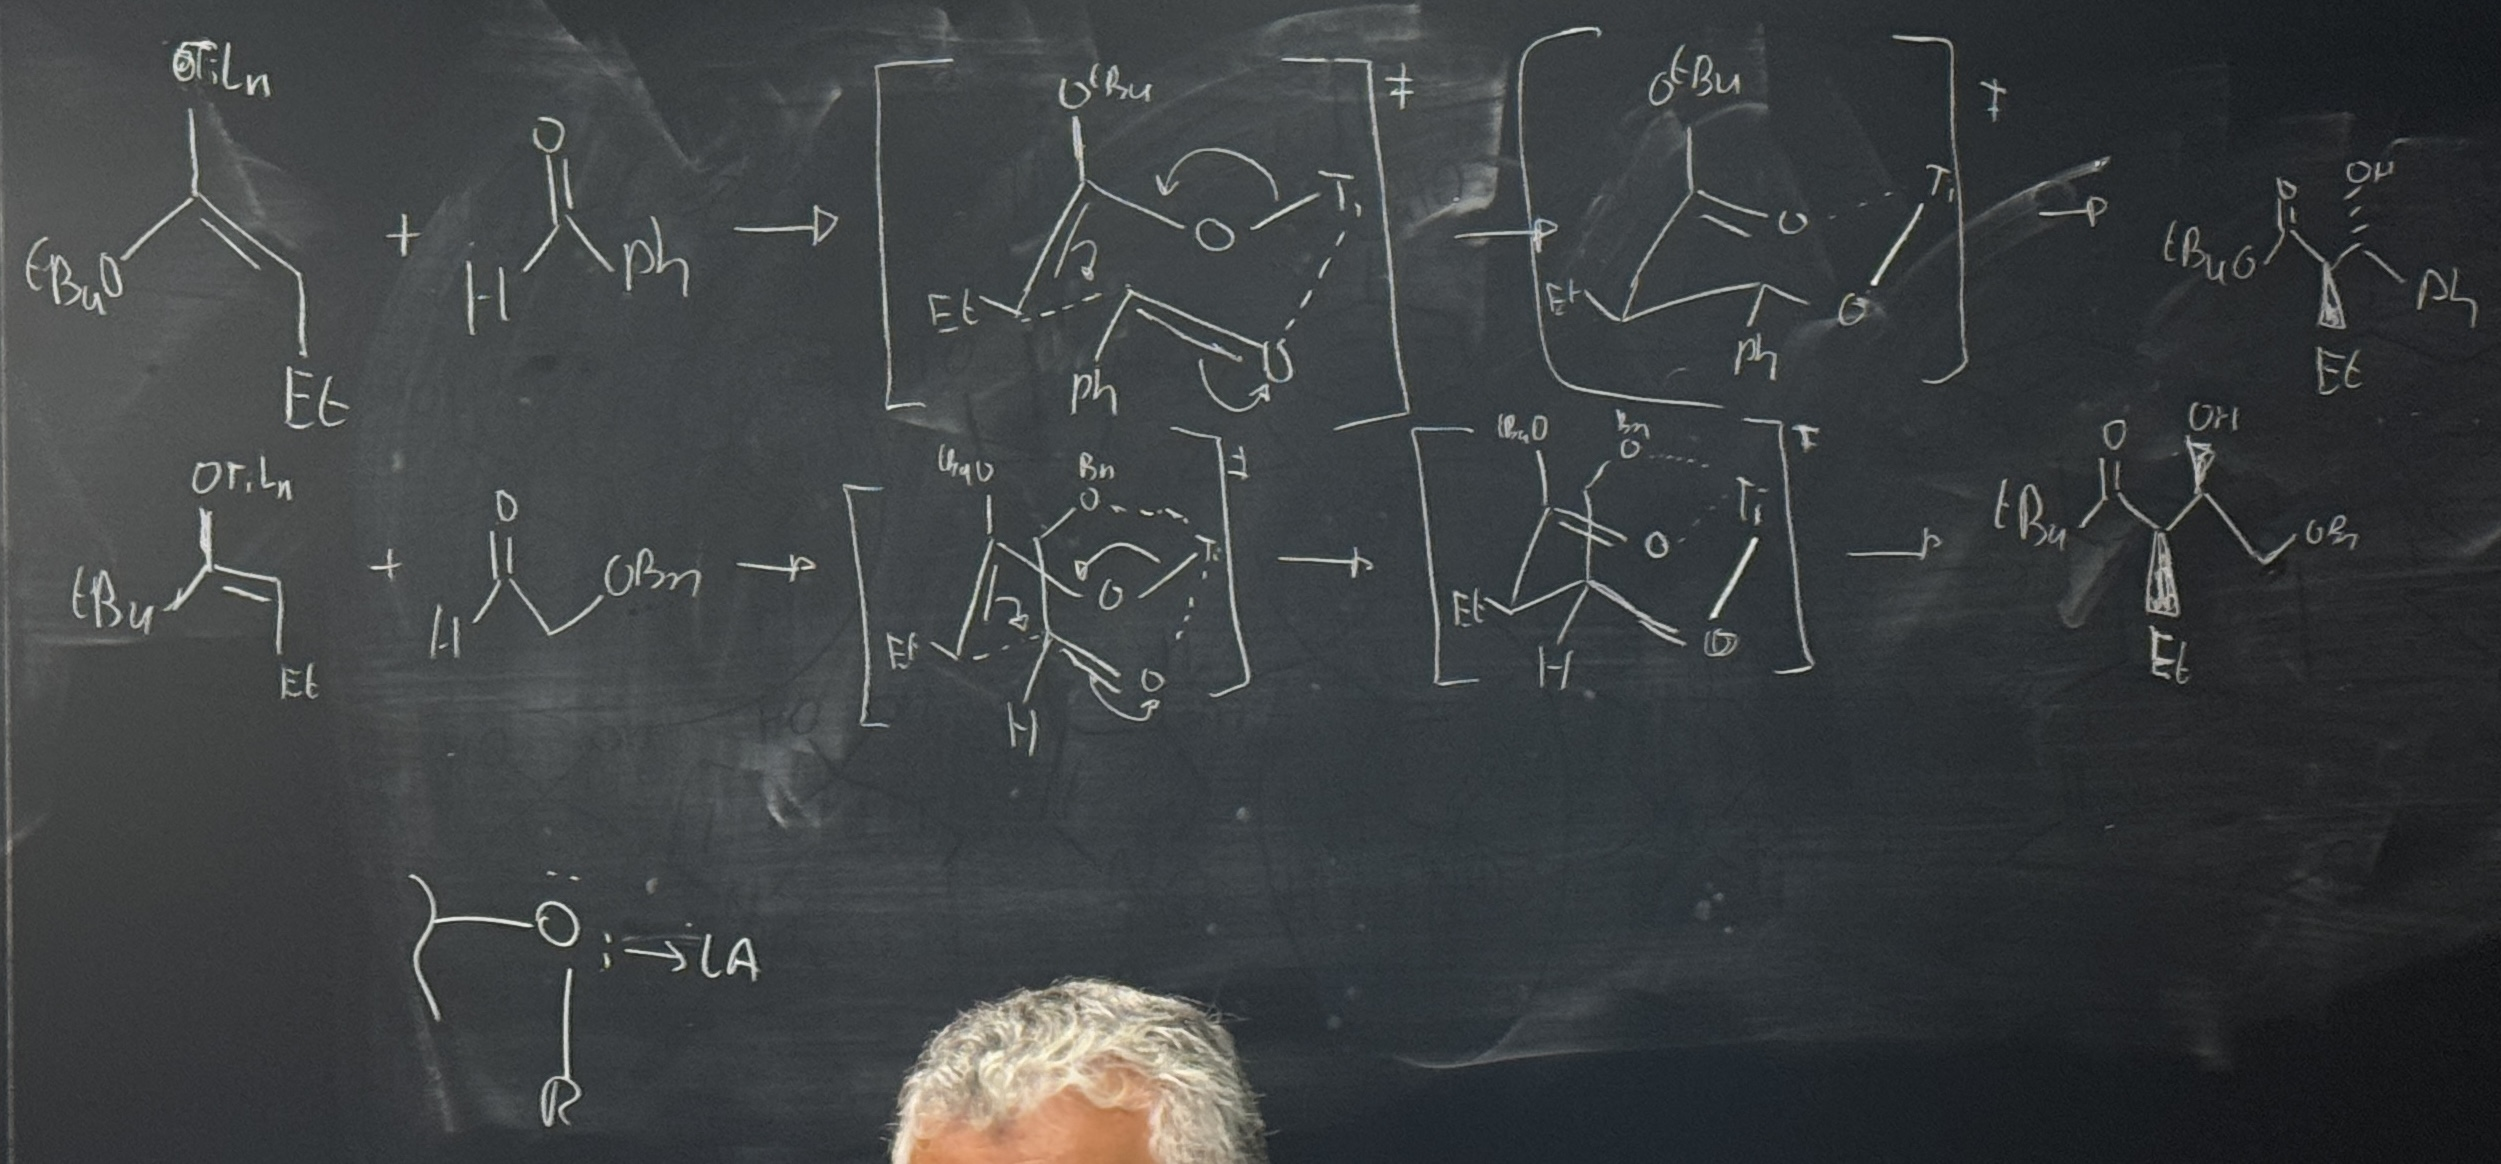
\includegraphics[width=0.8\linewidth]{MPSet3Q6S.JPG}
        \caption{Movassaghi PSet 3, Q6 solution.}
        \label{fig:MPSet3Q6S}
    \end{figure}
    \pagebreak
    \item Look over 5.43 - Advanced Organic Chemistry MIT OCW in the weeks before I begin 5.511!!
\end{itemize}




\end{document}